 \documentclass[letterpaper,11pt]{article}
\usepackage{tgpagella}
\usepackage[utf8]{inputenc}
\usepackage{graphicx}
\usepackage{fullpage,paralist}
\usepackage{amsmath, amssymb, amsthm}
\usepackage{comment,hyperref}
\usepackage{thmtools}
\usepackage{tikz}
\usepackage{pgfplots}
\usepackage{varwidth}
\pgfplotsset{compat=1.10}
\usepgfplotslibrary{fillbetween}
\usetikzlibrary{backgrounds}
\usetikzlibrary{patterns}


\newcommand{\psf}{\mathsf{P}}

\begin{document}
	
	\textbf{Ejemplo}
\begin{center}
	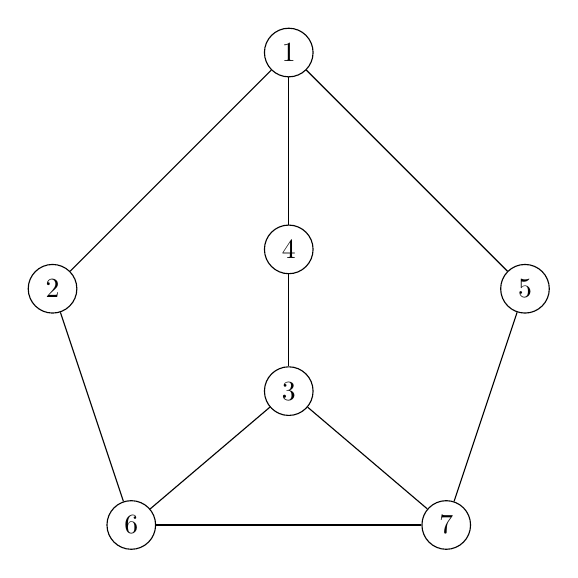
\begin{tikzpicture}
	\node[draw,circle] (1) at (3,6) {1};
	\node[draw,circle] (2) at (0,3) {2};
	\node[draw,circle] (3) at (3,1.7) {3};
	\node[draw,circle] (4) at (3,3.5) {4};
	\node[draw,circle] (5) at (6,3) {5};
	\node[draw,circle] (6) at (1,0) {6};
	\node[draw,circle] (7) at (5,0) {7};
	%
	\draw[-] (1) -- (2);
	\draw[-] (1) -- (4);
	\draw[-] (1) -- (5);
	\draw[-] (2) -- (6);
	\draw[-] (4) -- (3);
	\draw[-] (6) -- (3);
	\draw[-] (7) -- (3);
	\draw[-] (7) -- (6);
	\draw[-] (7) -- (5);
	\end{tikzpicture}
\end{center}

\[
\psf(u,v)= \left(
\begin{array}{cccccccccccc}
0 & 1/4 & 0 & 1/4 & 1/4 & 0  & 0 &1/4 & 0 & 0 & 0\\
1/3& 0 & 0 & 0 & 0 & 1/3  & 0 &0 & 1/3 & 0 & 0\\
0& 0 & 0 & 1/3 & 0 & 1/3  & 1/3 &0 & 0 & 0 & 0\\
1/3& 0 & 1/3 & 0 & 0 &  0 & 0 &0 & 0 & 1/3 & 0\\
1/3& 0 & 0 & 0 & 0 &  0 & 1/3  &0 & 0 & 0 & 1/3\\
0& 1/3 & 1/3 & 0 & 0 & 0  & 1/3  &0 & 0 & 0 & 0\\
0& 1/3 & 0 & 0 & 1/3 & 1/3  & 0  &0 & 0 & 0 & 0\\
1& 0 & 0 & 0 & 0 & 0  & 0  &0 & 0 & 0 & 0\\
0& 1 & 0 & 0 & 0 & 0  & 0  &0 & 0 & 0 & 0\\
0& 0 & 0 & 1 & 0 & 0  & 0  &0 & 0 & 0 & 0\\
0& 0 & 0 & 0 & 1 & 0  & 0  &0 & 0 & 0 & 0\\
\end{array} \right)
\]

\begin{itemize}
	\item $v_0=3$, $A=\{6,7,8,9,10,11\}$
	\begin{align*}
	g(1)&=1/9\\
	g(2)&=1/27\\
	g(4)&=10/27\\
		g(5)&=1/27\\
		\end{align*}
		\item $v_0=6$, $A=\{3,7,8,9,10,11\}$
		\begin{align*}
		g(1)&=1/9\\
		g(2)&=10/27\\
		g(4)&=1/27\\
		g(5)&=1/27\\
	\end{align*}
	\item $v_0=7$, $A=\{3,6,8,9,10,11\}$
	\begin{align*}
	g(1)&=1/9\\
	g(2)&=1/27\\
	g(4)&=1/27\\
	g(5)&=10/27\\
	\end{align*}
	\item $v_0=8$, $A=\{3,6,7,9,10,11\}$
\begin{align*}
g(1)&=1/3\\
g(2)&=1/9\\
g(4)&=1/9\\
g(5)&=1/9\\
\end{align*}
\item $v_0=9$, $A=\{3,6,7,8,10,11\}$
\begin{align*}
g(1)&=1/9\\
g(2)&=10/27\\
g(4)&=1/27\\
g(5)&=1/27\\
\end{align*}
\item $v_0=10$, $A=\{3,6,7,8,9,11\}$
\begin{align*}
g(1)&=1/9\\
g(2)&=1/27\\
g(4)&=10/27\\
g(5)&=1/27\\
\end{align*}
\item $v_0=11$, $A=\{3,6,7,8,9,10\}$
\begin{align*}
g(1)&=1/9\\
g(2)&=1/27\\
g(4)&=1/27\\
g(5)&=10/27\\
\end{align*}
\end{itemize}
\end{document}